\noindent Esta parte presenta los resultados en el orden de las preguntas de la
sección~\ref{sec:intro}. Cada sección explica qué se hizo y cómo leer sus figuras, y termina con
un recuadro que responde una pregunta. Todos los resultados se obtuvieron sobre las dos
consultas de prueba (1161 y 1180~s), con las cotas archivadas del actuador, salvo cuando se
indica otra cosa.

%======================================================================
\section{La réplica del ROM es exacta (F1)}\label{sec:replica}
%======================================================================
\paragraph{Qué se hizo y por qué.} Para optimizar con derivadas hace falta el modelo escrito
como ecuaciones en un lenguaje que pueda derivarlas, y no como un diagrama de bloques en
Simulink. F0 extrajo el ROM término a término desde los bloques del archivo de Simulink, y F1 lo
programó en Julia (\code{julia/SMDFRROM.jl}). Antes de usar esa réplica hay que demostrar que
calcula \emph{lo mismo} que Simulink.

\paragraph{Cómo se validó.} La validación reconstruye una consulta igual que el lazo: se inyecta
el estado del HRM en $t_q-10$~s, se simulan 10~s de calentamiento y luego los 26 pasos del
horizonte, con las mismas entradas. Se compararon tres variantes del integrador:

\begin{table}[H]\centering\small
\begin{tabularx}{\linewidth}{@{}Y r r@{}}\toprule
Esquema de la réplica & Error máx.\ en el horizonte & Error máx.\ en toda la ventana\\\midrule
\code{ode1be} (una iteración de Newton), entradas en $t_{n+1}$ & $\mathbf{2.2\cdot10^{-6}}$~K & $1.1\cdot10^{-4}$~K\\
\code{ode1be}, entradas en $t_n$ & $7.2\cdot10^{-2}$~K & $7.2\cdot10^{-2}$~K\\
Euler implícito convergido, entradas en $t_{n+1}$ & $3.7\cdot10^{-4}$~K & 0.88~K\\\bottomrule
\end{tabularx}
\caption{Error de la réplica frente a Simulink en la consulta de 1180~s.}
\end{table}
\noindent La tabla enseña dos cosas. Primero, los detalles numéricos importan: tomar las entradas
al principio del paso en lugar de al final cambia el resultado en 0.07~K, casi cinco órdenes de
magnitud más que el error de la versión correcta. Segundo, Euler implícito convergido se aparta
de \code{ode1be} en el transitorio de calentamiento, donde el estado inyectado desde el HRM
produce un salto rápido, pero no en el horizonte. Por eso el NLP parte del estado en
$t_q-\Delta t$, ya pasado el calentamiento.

\begin{figure}[H]\centering
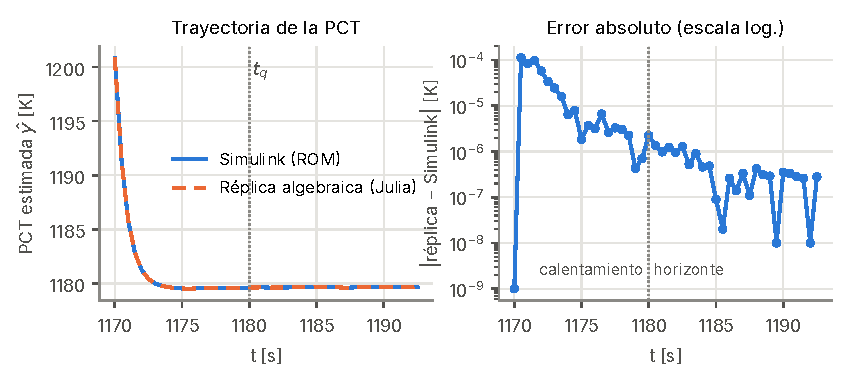
\includegraphics[width=\linewidth]{figures/fig_replica.pdf}
\caption{Consulta de 1180~s. Izquierda: PCT estimada por Simulink y por la réplica. Derecha:
error absoluto. Con el mismo esquema que Simulink (\code{ode1be}, una iteración de Newton,
entradas en $t_{n+1}$), el error es de $2\cdot10^{-6}$~K en el horizonte y de
$10^{-4}$~K en el transitorio del calentamiento. En 1161~s es de $1.6\cdot10^{-6}$~K.}
\end{figure}

\takeaway{La réplica es un sustituto exacto de Simulink, con derivadas disponibles. Todo
lo que sigue se apoya en ella.}


%======================================================================
\section{El problema determinista se resuelve en tiempo real (F2, F3)}\label{sec:resolucion}
%======================================================================

\subsection{La solución del NLP}
El NLP (N3) se resuelve en $\sim0.05$~s. Las cuatro inicializaciones probadas (acción de
LJ, cota inferior, cota superior y punto medio) llegan al mismo óptimo.

\begin{figure}[H]\centering
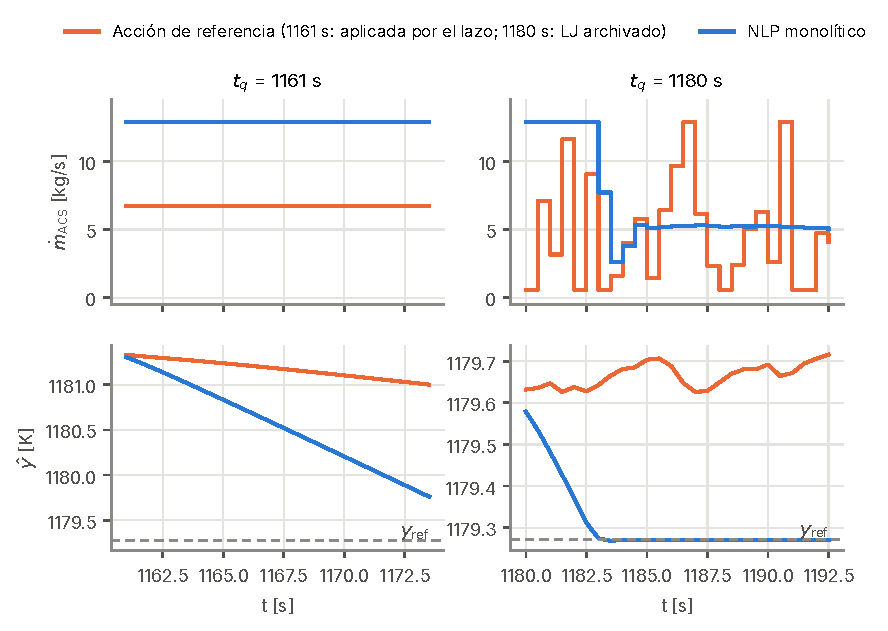
\includegraphics[width=\linewidth]{figures/fig_f2_nlp.pdf}
\caption{Acción (arriba) y PCT estimada (abajo) del NLP frente a la acción de referencia
archivada. En 1180~s el NLP satura durante 3~s y luego sigue la referencia exactamente. En
1161~s el óptimo es la esquina $u=u_{\rm max}$ durante todo el horizonte, y aun así la PCT
no alcanza la referencia: la cota del actuador limita el resultado.}
\end{figure}

\paragraph{Por qué ``saturar y luego seguir''.} La función de transferencia del modelo
lineal, de $\mdot_{\rm ACS}$ a $\hat y$, es $G(s)\approx G_M/s$, con
$\partial\hat y/\partial\Delta M=-1.6\cdot10^{-2}$~K/kg: el ACS actúa a través de un
integrador puro, el inventario. Conviene acumular inventario lo antes posible. Con la cota
archivada, la autoridad sobre el horizonte es de unos 150~kg, es decir, $\approx-2.4$~K
como máximo sobre la PCT.

\subsection{N1 y N2 frente a N3}
\begin{figure}[H]\centering
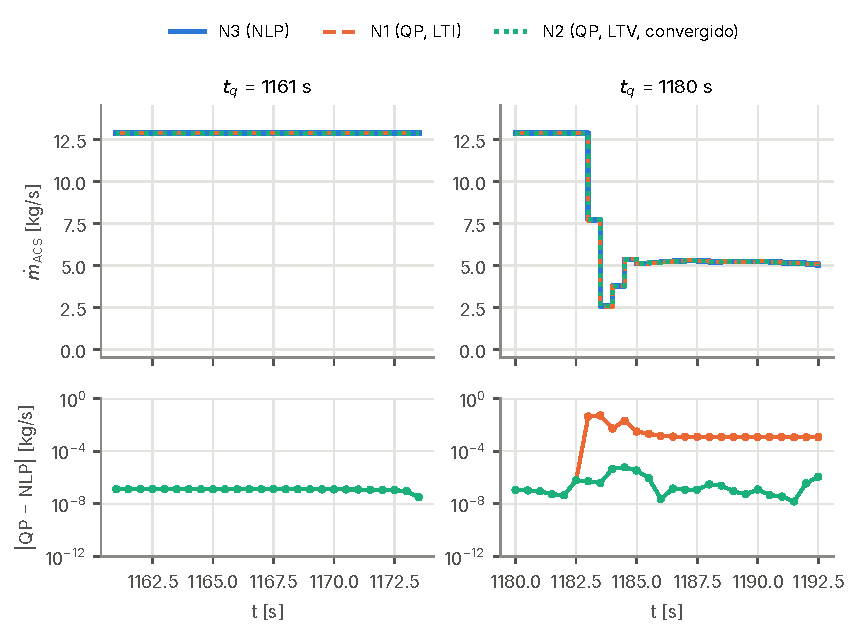
\includegraphics[width=\linewidth]{figures/fig_nlp_vs_qp.pdf}
\caption{Arriba: acciones de N3 (NLP), N1 y N2 convergido. Abajo: diferencia con el NLP,
en escala logarítmica. En 1161~s coinciden a $10^{-7}$~kg/s. En 1180~s, N1 se separa hasta
0.054~kg/s justo donde el óptimo deja de saturar, mientras que N2 converge al NLP a
$6\cdot10^{-6}$~kg/s.}
\end{figure}

\begin{figure}[H]\centering
\begin{minipage}{0.56\linewidth}
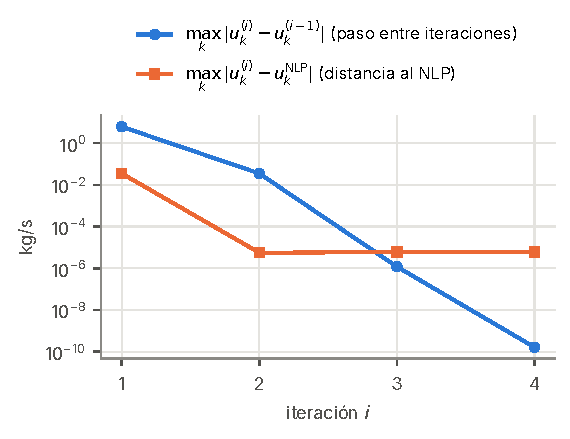
\includegraphics[width=\linewidth]{figures/fig_sqp.pdf}
\end{minipage}\hfill
\begin{minipage}{0.4\linewidth}\small
\captionof{figure}{Convergencia de N2 en 1180~s. El paso entre iteraciones cae de forma
superlineal (6.1, $3.5\cdot10^{-2}$, $1.2\cdot10^{-6}$, $1.6\cdot10^{-10}$~kg/s), y la
distancia al NLP se estabiliza en $6\cdot10^{-6}$~kg/s, que es la tolerancia del propio
NLP. En 1161~s converge en una iteración.}
\end{minipage}
\end{figure}

\begin{table}[H]\centering\footnotesize\setlength{\tabcolsep}{4pt}
\begin{tabularx}{\linewidth}{@{}l Y r r r r@{}}\toprule
Modelo & Forma, solver & Var. & Tiempo [s] & Brecha dual & Máx. dif. con NLP [kg/s]\\\midrule
\multicolumn{6}{@{}l}{\emph{$t_q=1180$~s}}\\
N3 & disperso, Ipopt & 519 & 0.055 & --- & ---\\
N1 & disperso / condensado, Clarabel & 519 / 77 & 0.037 / 0.010 & $\sim10^{-12}$ & $5.4\cdot10^{-2}$\\
N2 & condensado, Clarabel (por QP) & 77 & 0.010 & $<10^{-11}$ & $5.9\cdot10^{-6}$\\
\multicolumn{6}{@{}l}{\emph{$t_q=1161$~s}}\\
N3 & disperso, Ipopt & 519 & 0.048 & --- & ---\\
N1, N2 & condensado, Clarabel & 77 & 0.009 & $\sim4\cdot10^{-11}$ & $1.3\cdot10^{-7}$\\\bottomrule
\end{tabularx}
\caption{Resolución de los QP. La brecha dual certifica que cada QP quedó resuelto
(proposición~\ref{prop:dual}).}
\end{table}

\begin{figure}[H]\centering
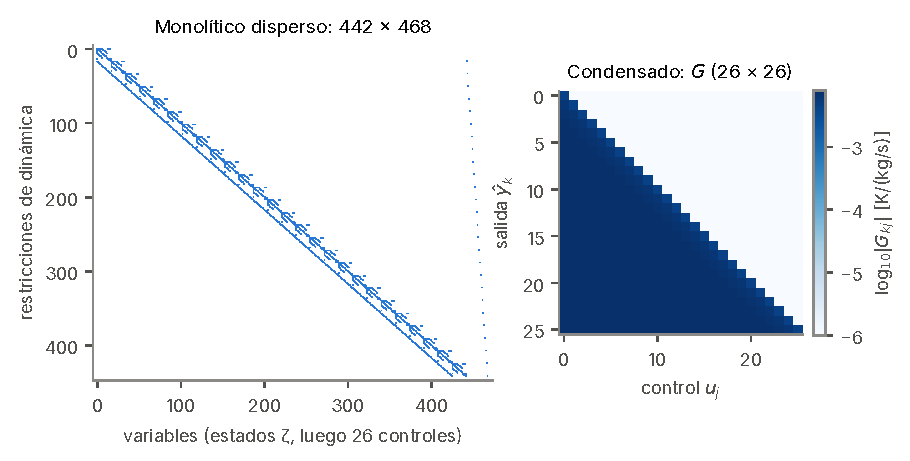
\includegraphics[width=\linewidth]{figures/fig_structure.pdf}
\caption{Estructura del QP de N1. Izquierda: restricciones de la forma dispersa, con bloques
$(I-\Delta tA)$ en la diagonal, $-I$ en la subdiagonal y una columna por control. Derecha:
matriz condensada $G$, triangular inferior y con columnas casi constantes, que son la
huella del integrador del inventario.}
\end{figure}

\takeaway{\textbf{Respuesta a Q1.} Sí. El NLP resuelve P0 en $\sim0.05$~s y el QP condensado
en $\sim10$~ms, frente a $\sim800$~s de LJ, y la solución no depende de semillas. La
linealización reproduce la decisión del NLP: N2 coincide con él y N1 se aparta poco. Una
versión anterior de N2 se estancaba a 0.02~kg/s del NLP. La causa estaba en su
implementación, que trabajaba con términos constantes del orden de $10^{16}$; la
formulación en desviaciones lo corrigió.}


%======================================================================
\section{¿Es el óptimo global? Certificación del P0 no lineal (F3c)}\label{sec:certificacion}
%======================================================================

\subsection{Planteamiento}
El problema que se certifica es N3 en \emph{espacio reducido}. Los estados se eliminan con
la simulación, $x_k=\Phi(x_{k-1},u_k)$, y el costo queda como función sólo del control:
$J^\star=\min_{u\in\mathcal U}J(u)$, con $\mathcal U=[\mdot_{\rm min},\mdot_{\rm max}]^{26}$.
$J$ se programó de forma genérica, de modo que se deriva \emph{a través de la simulación}.
En el paso implícito se resuelve Newton sobre valores y luego se hacen tres refinamientos
con números duales, lo que da derivadas primeras y segundas exactas. El costo reducido en
la solución coincide con el objetivo del NLP monolítico a $4\cdot10^{-8}$.

\begin{table}[H]\centering\small
\begin{tabularx}{\linewidth}{@{}l Y l@{}}\toprule
Paso & Pregunta & Tipo de resultado\\\midrule
1 & ¿La solución de Ipopt es un mínimo y no un punto de silla? & Prueba local\\
2 & ¿Cambia el óptimo con la discretización exacta de Simulink? & Consistencia\\
3 & ¿Hay otro óptimo mejor en la caja de control? & Evidencia global\\
4a & ¿Cuánto podría mejorarse, si el residuo no lineal está bien estimado? & Brecha semi-rigurosa\\
4b & ¿Cuánto podría mejorarse, con demostración? & \textbf{Brecha certificada}\\\bottomrule
\end{tabularx}
\caption{Las pruebas de la certificación.}
\end{table}

\subsection{Paso 1: la solución es un mínimo local estricto}
Se verificaron las tres condiciones de la proposición~\ref{prop:sosc}, con la hessiana
calculada por diferencias centrales del gradiente exacto.

\begin{table}[H]\centering\small
\begin{tabularx}{\linewidth}{@{}l Y Y@{}}\toprule
& $t_q=1180$~s & $t_q=1161$~s\\\midrule
Cotas activas / variables libres & 6 superiores / 20 & 26 superiores / 0\\
Máx. $|\partial J/\partial u|$ en las libres & $8.7\cdot10^{-10}$ & ---\\
Menor multiplicador de cota activa & $3.2\cdot10^{-4}$ & $4.2\cdot10^{-3}$\\
$\lambda_{\rm min}$ de la hessiana reducida & $4.3\cdot10^{-6}$ (condición $4.6\cdot10^3$) & --- (vértice)\\
Conclusión & mínimo local estricto & mínimo local estricto en un vértice\\\bottomrule
\end{tabularx}
\caption{Paso 1: condiciones de la proposición~\ref{prop:sosc}.}
\end{table}

\subsection{Paso 2: la discretización de Simulink da el mismo óptimo}
Se resolvió P0 con la discretización \code{ode1be} (Ipopt en espacio reducido, con
gradiente exacto). Su óptimo está a $4.5\cdot10^{-9}$ (1180~s) y $6.8\cdot10^{-7}$ (1161~s)
del obtenido con Euler implícito convergido, con la misma primera acción. Las dos
definiciones de P0 son equivalentes a efectos prácticos.

\subsection{Paso 3: no aparece ningún óptimo mejor}
\begin{itemize}
  \item \textbf{Multistart} del NLP desde unos 590 arranques: aleatorios uniformes,
        caminatas aleatorias, constantes, bang-bang, alternados y, en 1180~s, las soluciones
        de LJ y GA. Todos convergen al mismo óptimo, a $\le5\cdot10^{-6}$~kg/s.
  \item \textbf{Evolución diferencial} sin derivadas (población 60, 1500 generaciones,
        90\,060 evaluaciones): queda a $+2.4\cdot10^{-7}$ del NLP en 1180~s y lo iguala en
        1161~s.
  \item \textbf{Convexidad}: valores propios de $\nabla^2J$ en 300 puntos de la caja
        (figura~\ref{fig:hess}).
\end{itemize}

\begin{figure}[H]\centering
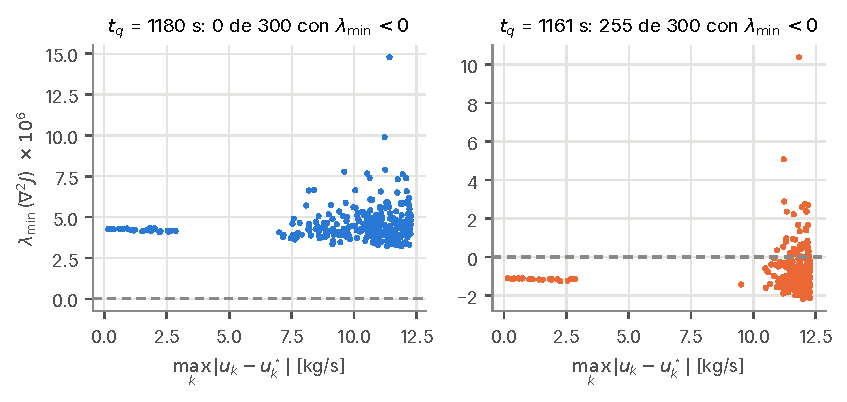
\includegraphics[width=\linewidth]{figures/fig_hessian.pdf}
\caption{Menor valor propio de la hessiana del costo en 300 puntos de la caja. En 1180~s es
positivo en todos. En 1161~s es levemente negativo en 255 puntos (hasta $-2\cdot10^{-6}$, un
0.006\,\% de $\lambda_{\rm max}$), también cerca del óptimo. Eso no contradice el paso 1: allí
las 26 variables están en su cota con multiplicadores positivos, y las cotas bloquean la
dirección de curvatura negativa.}
\label{fig:hess}
\end{figure}

\noindent La evidencia es fuerte, pero no es una prueba, y la no convexidad de 1161~s
muestra que no se puede suponer convexidad. Hace falta una cota inferior.

\subsection{Paso 4: una cota inferior del óptimo global}
La idea es construir una función $L(u)$ que quede por debajo de $J(u)$ en \emph{toda} la
caja y que sea convexa. Su mínimo es una cota inferior de $J^\star$.

\begin{proposicion}[Cota inferior por relajación del residuo]\label{prop:lb}
Sea $a(u)=\hat y(u_c)+G(u-u_c)$ un modelo afín cualquiera de la salida y
$e(u)=\hat y(u)-a(u)$ su residuo. Si $|e_k(u)|\le\varepsilon_k$ para todo $u\in\mathcal U$,
entonces la función
\[
L(u)=\sum_k\big(|a_k(u)-y_{\rm ref}|-\varepsilon_k\big)_+^2
+\lambda_m\sum_k\big[|u_{k+1}-u_k|-\Delta\mdot\big]_+^2
+\lambda_{\rm pct}\sum_k\big[a_k(u)-\varepsilon_k-U_y\big]_+^2
\]
es convexa, cumple $L(u)\le J(u)$ en $\mathcal U$, y $LB=\min_{u\in\mathcal U}L(u)\le J^\star$.
\end{proposicion}
\begin{proof}
Como $\hat y_k=a_k+e_k$ con $|e_k|\le\varepsilon_k$, se tiene
$|\hat y_k-y_{\rm ref}|\ge|a_k-y_{\rm ref}|-\varepsilon_k$, y como el lado izquierdo es no
negativo, $(\hat y_k-y_{\rm ref})^2\ge(|a_k-y_{\rm ref}|-\varepsilon_k)_+^2$. También
$\hat y_k-U_y\ge a_k-\varepsilon_k-U_y$ y $[\cdot]_+^2$ es creciente. El término de la rampa
depende sólo de $u$ y es idéntico. Sumando, $L\le J$. Cada término es la composición de una
función convexa no decreciente, $t\mapsto(t)_+^2$, con una función convexa de $u$ (el valor
absoluto de una función afín, o una función afín), así que $L$ es convexa. Por último,
$LB=\min L\le L(u^\star)\le J(u^\star)=J^\star$, con $u^\star$ el óptimo global.
\end{proof}
\noindent $\min L$ se escribe como un QP: $t_k\ge0$, $t_k\ge\pm(a_k-y_{\rm ref})-\varepsilon_k$
y se minimiza $\sum t_k^2$. Clarabel lo resuelve con su cota dual. Lo único difícil es
obtener $\varepsilon_k$.

\subsubsection{Paso 4a: residuo estimado por muestreo (semi-riguroso)}
$\varepsilon_k$ se estima con 3000 puntos aleatorios, 63 patrones extremos y una
maximización adversaria de $\pm e_k$ con Ipopt. La búsqueda adversaria no superó al
muestreo en ningún paso. Con $u_c=u^\star$, la brecha es de \textbf{0.30\,\% (1180~s) y 1.2\,\%
(1161~s)}, y de 0.59\,\% y 2.4\,\% si $\varepsilon$ se duplica por seguridad. Es
semi-rigurosa porque el muestreo podría no encontrar el peor residuo.

\subsubsection{Paso 4b: residuo demostrado con aritmética de intervalos}
\begin{proposicion}[Encierro del resto no lineal]\label{prop:taylor}
Sea $\delta_k(u)=x_k(u)-x^c_k=T_k\Delta u+r_k$, con $T_k$ la parte lineal exacta. Si en el
paso $k$ una caja de intervalos $R$ cumple $\mathcal F_k(R)\subseteq R$, donde
\[
\mathcal F_k(R)=C_k\Big(r_{k-1}+h\big([A](Z_k)-A^c_k\big)\big(T_k[\Delta u]+R\big)-\mathrm{res}_k-D_k[\Delta u]\Big)+(I-C_kM^c_k)R,
\]
$Z_k=x^c_k+T_k[\Delta u]+R$, $M^c_k=I-hA^c_k$ y $C_k\approx(M^c_k)^{-1}$, y si cada paso de
Euler implícito tiene solución única cerca de la nominal, entonces $r_k(u)\in\mathcal F_k(R)$
para todo $u\in\mathcal U$.
\end{proposicion}
\begin{proof}[Idea de la demostración]
Restando el paso implícito de la trayectoria real y el de la nominal, y aplicando el
teorema del valor medio a $f$ fila por fila, $M^c_k\delta_k=\delta_{k-1}+hB\Delta u_k
+h(A(\xi)-A^c_k)\delta_k-\mathrm{res}_k$, con $A(\xi)$ evaluado en puntos del segmento que
une ambas trayectorias. Si $\delta_k\in T_k[\Delta u]+R$, esos puntos están en $Z_k$ y
$A(\xi)\in[A](Z_k)$. Restando la parte lineal, el resto cumple $r_k\in\mathcal F_k(R)$.
Como $\mathcal F_k$ lleva $R$ dentro de sí misma, el teorema de Brouwer asegura que existe
una solución en $R$, y por unicidad es la verdadera. Los defectos de punto flotante
($\mathrm{res}_k$, $D_k$ y $I-C_kM^c_k$) se encierran con intervalos de redondeo dirigido.
\end{proof}

\noindent El residuo de salida es entonces
$e_k\in S_{T_w}r_k[T_w]+\tfrac12[p_4''](\cdot)\Delta u_k^2$, y $\varepsilon_k$ es su mayor
valor absoluto. Se verificó que el jacobiano por intervalos contiene los 1300 jacobianos
muestreados por consulta, sin ninguna violación; que la caja $R$ se acepta en los 26 pasos
con dos iteraciones; y que el $\varepsilon$ riguroso supera siempre al residuo muestreado
del mismo modelo afín.

\begin{table}[H]\centering\small
\begin{tabular}{@{}lccc@{}}\toprule
Centro $u_c$ del modelo afín & $\varepsilon_{26}$ riguroso / muestreado & Brecha 1180~s & Brecha 1161~s\\\midrule
$u^\star$ (solución del NLP) & 0.50 / 0.010~K; 1.32 / 0.038~K & 4.86\,\% & 20.85\,\%\\
Punto medio de la caja & 0.47 / 0.009~K; 0.48 / 0.010~K & \textbf{2.34\,\%} & \textbf{11.44\,\%}\\\bottomrule
\end{tabular}
\caption{Brecha certificada $(UB-LB)/UB$ sobre toda la caja de control. Con el centro en el
punto medio, $LB=0.23834$ (1180~s) y $LB=42.533$ (1161~s).}
\end{table}

\begin{figure}[H]\centering
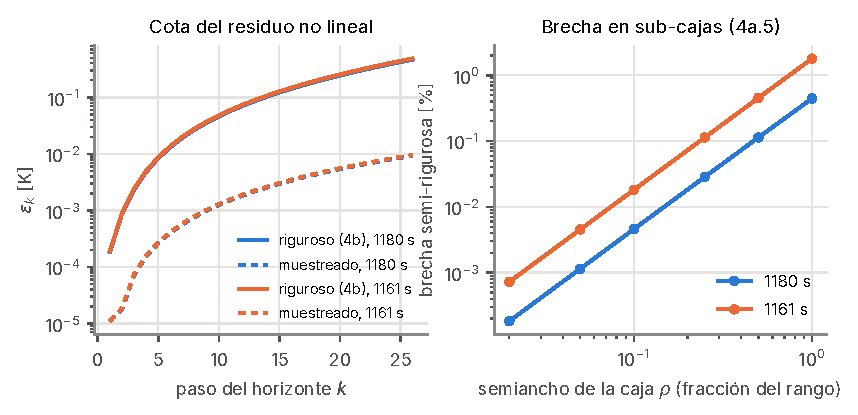
\includegraphics[width=\linewidth]{figures/fig_bounds.pdf}
\caption{Izquierda: cota del residuo por paso del horizonte, rigurosa frente a muestreada.
Derecha: brecha semi-rigurosa en sub-cajas de semiancho $\rho$ alrededor de $u^\star$, que
baja como $\rho^2$, como el resto de una expansión de Taylor.}
\end{figure}

\takeaway{\textbf{Respuesta a Q2.} La solución del NLP es un mínimo local estricto, es el
único óptimo encontrado, y el óptimo global está demostradamente en $[0.23834,\ 0.24403]$
(1180~s) y en $[42.53,\ 48.03]$ (1161~s). Es decir, la solución está a menos del 2.3\,\% y
del 11.4\,\% del óptimo global. La cota rigurosa sobreestima el residuo real entre 16 y 50
veces, porque acota el término de segundo orden como un producto de cajas e ignora que las
26 direcciones de control mueven el estado casi en una sola dirección. Ajustarla es el
próximo paso; la evidencia de los pasos 1--3 indica que la brecha real es $\approx0$.}


%======================================================================
\section{¿Cuál método es mejor, y por cuánto?}\label{sec:comparacion}
%======================================================================

\subsection{Métodos comparados}
\begin{table}[H]\centering\footnotesize\setlength{\tabcolsep}{3pt}
\begin{tabularx}{\linewidth}{@{}>{\raggedright\arraybackslash}p{24mm} Y Y Y r@{}}\toprule
Método & Modelo con el que decide & Formulación & Algoritmo & Tiempo\\\midrule
N3, NLP & ROM no lineal, Euler implícito & Monolítica dispersa, 519 variables & Ipopt, hessiana exacta & 0.05~s\\
N3 sobre \code{ode1be} & ROM no lineal, \code{ode1be} & Espacio reducido, 26 variables & Ipopt, gradiente exacto, L-BFGS & 2.5--10~s\\
N2 & ROM linealizado por paso, iterado & QP condensado, 77 variables & SQP + Clarabel & 10~ms por QP\\
N1 & ROM linealizado en un punto & QP condensado, 77 variables & Clarabel & 0.01~s\\
Evolución diferencial & ROM no lineal & 26 variables & Sin derivadas, 90\,060 evaluaciones & 90~s\\
LJ corregido & ROM en Simulink & 26 corrientes & Luus--Jaakola ($R=24$, $\gamma=0.9$, $M=5$), 721 evaluaciones & $\approx800$~s\\
GA & ROM en Simulink & 26 corrientes & Genético $20\times20$, 420 evaluaciones & $\approx615$~s\\
Lazo archivado & Lazo original, previo a la corrección de LJ & --- & --- & ---\\\bottomrule
\end{tabularx}
\caption{Métodos comparados. Los tiempos de LJ y GA son de MATLAB/Simulink; los demás, de
Julia.}
\end{table}

\subsection{Cómo se compara}
\begin{enumerate}
  \item \textbf{Misma vara.} El control de cada método se evalúa con el costo P0 sobre el
        ROM \emph{no lineal}, en las dos discretizaciones (dan el mismo ordenamiento). Nunca
        se usa el objetivo interno de cada solver: por ejemplo, el QP N1 predice 47.81 en
        1161~s, pero su control cuesta 48.03 en el modelo no lineal.
  \item \textbf{Mismas condiciones.} Mismo estado inicial, mismo pronóstico de fuga, misma
        referencia, mismas cotas del actuador y misma rampa. Las corrientes de LJ y GA se
        convierten a caudal con el mapa de la bomba, y su costo recalculado coincide con el
        medido en Simulink.
  \item \textbf{Calidad garantizada.} Con la cota certificada de la sección anterior, el
        exceso real de cada decisión sobre el óptimo global queda en el intervalo de la
        proposición~\ref{prop:exceso}.
\end{enumerate}

\subsection{Resultados}
\begin{table}[H]\centering\footnotesize\setlength{\tabcolsep}{3pt}
\begin{tabular}{@{}lrrrrr@{}}\toprule
& \multicolumn{3}{c}{$t_q=1180$~s} & \multicolumn{2}{c}{$t_q=1161$~s}\\
\cmidrule(lr){2-4}\cmidrule(l){5-6}
Método & Costo & Exceso/mejor & Exceso garantizado & Costo & Exceso/mejor\\\midrule
N3, NLP & 0.244034 & 0 & 0 -- 2.4\,\% & 48.028 & 0\\
N3 sobre \code{ode1be} & 0.244034 & 0 & 0 -- 2.4\,\% & 48.028 & 0\\
N2, QP iterado & 0.244034 & 0 & 0 -- 2.4\,\% & 48.028 & 0\\
N1, QP & 0.244040 & +0.0026\,\% & 0.0026 -- 2.4\,\% & 48.028 & 0\\
Evolución diferencial & 0.244034 & +0.0001\,\% & 0.0001 -- 2.4\,\% & 48.028 & 0\\
LJ corregido (3 semillas) & 0.313 -- 0.381 & +28 a +56\,\% & 28 -- 60\,\% & --- & ---\\
GA (2 semillas) & 0.349 -- 0.353 & +43 a +45\,\% & 43 -- 48\,\% & --- & ---\\
Lazo archivado & 4.081 & +1572\,\% & 1572 -- 1612\,\% & 94.45 & +97\,\%\\\bottomrule
\end{tabular}
\caption{Costo sobre el ROM no lineal de la decisión de cada método. En 1161~s el exceso
garantizado de N1--N3 es 0--12.9\,\% y el del lazo archivado, 97--122\,\%; LJ y GA no tienen
corridas completas en esa consulta.}
\end{table}

\begin{figure}[H]\centering
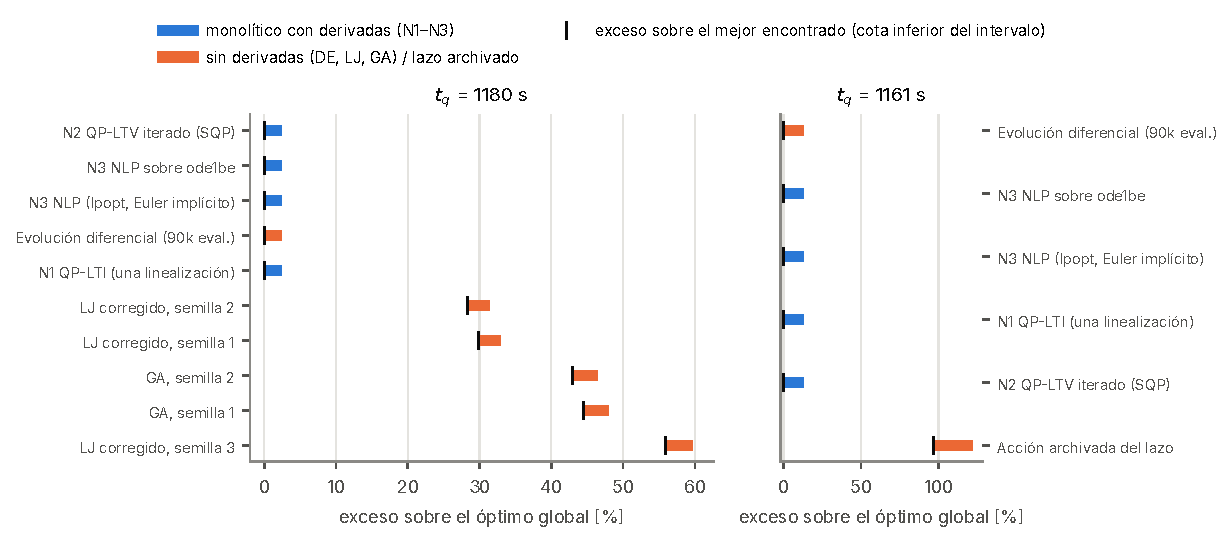
\includegraphics[width=\linewidth]{figures/fig_decisions.pdf}
\caption{Intervalo de exceso garantizado de cada decisión. La marca negra es el exceso sobre
el mejor encontrado y la barra llega hasta el límite que fija la cota certificada. En
1180~s se omite el lazo archivado (1572--1612\,\%).}
\end{figure}

\takeaway{\textbf{Respuesta a Q3.} N3 y N2 son los mejores y empatan: dan la misma decisión.
N1 cuesta un 0.0026\,\% más en 1180~s y lo mismo en 1161~s; es el más rápido y el único QP
convexo certificable, así que es el candidato natural para tiempo real. Los cuatro
aplican la misma primera acción (56.75~A). LJ y GA quedan dominados con garantía: su exceso
sobre el óptimo global es de al menos 28\,\% y 43\,\%, y tardan unas $10^4$ veces más. La
acción del lazo archivado era la peor: +1572\,\% en 1180~s y +97\,\% en 1161~s.}


%======================================================================
\section{¿El riesgo del pronóstico cambia la decisión? (F4)}\label{sec:riesgo}
%======================================================================
El ensamble MC-dropout de la BiLSTM se regeneró sin MATLAB, reconstruyendo su ventana de
entrada desde las trayectorias archivadas. La muestra que usó el lazo archivado cae dentro
del ensamble. Además se halló que el lazo usaba \code{N\_par = 1}: decidía con
\emph{una} realización aleatoria del dropout.

\begin{figure}[H]\centering
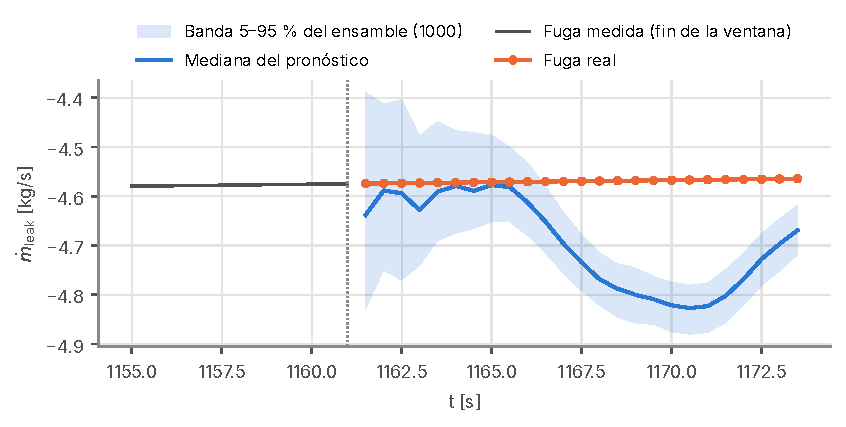
\includegraphics[width=\linewidth]{figures/fig_forecast.pdf}
\caption{Pronóstico de la fuga en 1161~s frente a la fuga real del HRM, que queda en el borde
superior de la banda del 90\,\% o fuera de ella.}
\end{figure}

\begin{figure}[H]\centering
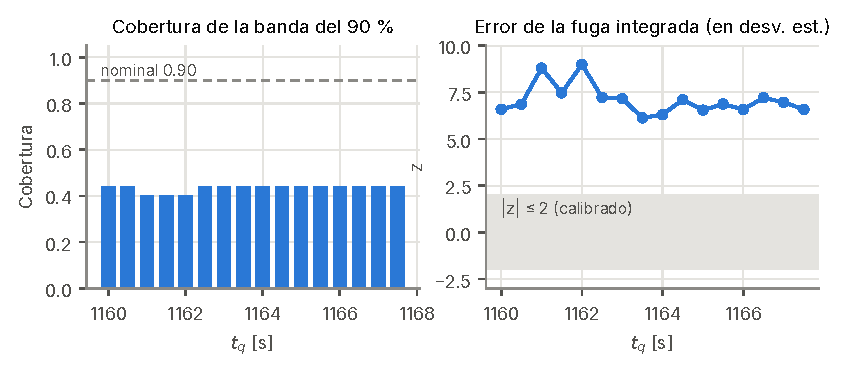
\includegraphics[width=\linewidth]{figures/fig_calibration.pdf}
\caption{Calibración en 16 consultas. La banda del 90\,\% cubre la fuga real sólo el 44\,\%
de las veces, y el error de la fuga integrada es de unas 7 desviaciones estándar.}
\end{figure}

\noindent El pronóstico está \textbf{sesgado} (unos 0.12~kg/s) y es
\textbf{sobreconfiado}. Pero su efecto sobre la PCT es mínimo: el error, integrado en el
horizonte (1.5~kg), equivale a $\approx0.025$~K, y la dispersión del ensamble a
$\approx0.003$~K, frente a una autoridad del actuador de $\approx2.4$~K.

\begin{table}[H]\centering\small
\begin{tabularx}{\linewidth}{@{}Y ll@{}}\toprule
& $t_q=1161$~s & $t_q=1180$~s\\\midrule
$u_0$ con fuga p05, p50, p95, sin dropout, real y SAA de 59 escenarios & todas 56.750~A & todas 56.750~A\\
Costo medio fuera de muestra (941 escenarios), rango entre variantes & 48.350 (idéntico) & 0.2443--0.2480\\
Tiempo: NLP determinista / SAA de dos etapas & 0.03 / 2.2~s & 0.03 / 2.3~s\\\bottomrule
\end{tabularx}
\caption{Decisiones bajo incertidumbre de pronóstico.}
\end{table}

\takeaway{\textbf{Respuesta a Q4.} No. Ninguna variante del riesgo de pronóstico cambia la
primera acción, ni siquiera cuando se amplía la autoridad del actuador para que no sature.
El SAA de dos etapas es viable en tiempo real ($\sim2$~s). El riesgo que sí podría mover
la decisión está en las fallas del ACS y en el desajuste entre el ROM y el HRM.}


%======================================================================
\section{¿Tienen base física las cotas del actuador?}\label{sec:actuador}
%======================================================================
Todos los resultados anteriores usan la cota archivada $u\in[56.69,56.75]$~A. Al revisarla
aparecieron tres hechos:
\begin{enumerate}
  \item El ACS es una inyección de reposición de inventario. La banda exploratoria de
        $\pm20$\,\% sobre el caudal primario nominal no sirve como restricción de la
        consulta: el propio LOCA ya la violó ($\mdot_c\approx0.6\,\mdot_{\rm nom}$), y
        recuperar $0.8\,\mdot_{\rm nom}$ exigiría unos 1700~kg.
  \item El modelo de la bomba (ECM) corresponde a una \emph{bomba principal}: ducto de
        $0.515\times0.515$~m, 15~kPa y 5543~kg/s a 2~m/s. El ACS usa el pie de su curva:
        0--13~kg/s en 0.06~A, con 1~mA equivalente a 0.2~kg/s.
  \item Por lo tanto, la cota en amperios no tiene significado físico. La cota defendible
        se expresa en kg/s, y debe acompañarse de un límite de rampa.
\end{enumerate}

\begin{figure}[H]\centering
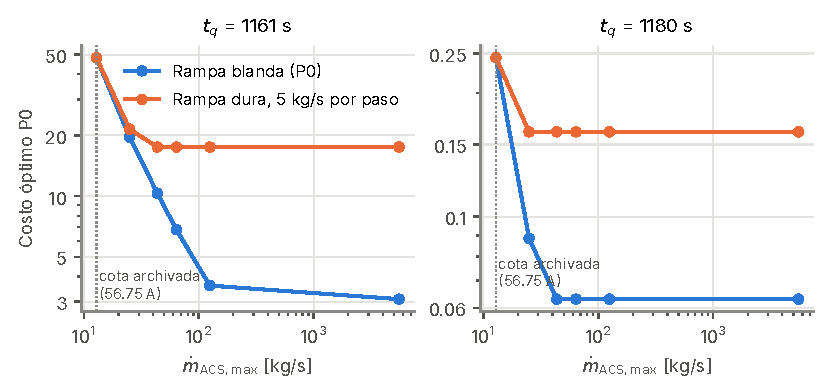
\includegraphics[width=\linewidth]{figures/fig_actuator.pdf}
\caption{Costo óptimo según la cota de caudal, con la rampa blanda de P0 o con una rampa dura
de 5~kg/s por paso.}
\end{figure}

\takeaway{\textbf{Respuesta a Q5.} No. Con una rampa dura, la cota de caudal deja de
importar desde 25--44~kg/s: la autoridad la fija la rampa. La pregunta física pasa de
``¿qué corriente máxima?'' a ``¿qué rampa admite la inyección?''. El costo óptimo en 1161~s
va de 3.1 a 48.4 según la cota y la rampa, así que este parámetro debe fijarse con el
equipo antes de sacar conclusiones operativas.}

